\documentclass[12pt, letterpaper]{article}
\usepackage{graphicx} % Required for inserting images
\usepackage{hyperref}
\usepackage{listings}
\usepackage{amssymb}
\usepackage{amsmath}
\usepackage[english]{babel}
\usepackage{amsfonts}
\usepackage{nicefrac, xfrac}
\usepackage[utf8]{inputenc}
\usepackage{mathtools}
\newcommand{\acc}{\\\hphantom{}\\}
\usepackage[dvipsnames]{xcolor}
\usepackage[titles]{tocloft} % Optional: Better control of the table of contents

\definecolor{light-gray}{gray}{0.95}
\newcommand{\code}[1]{\colorbox{light-gray}{\texttt{#1}}}
\newcommand{\codee}[1]{\colorbox{white}{\texttt{#1}}}
\usepackage[paper=a4paper,left=20mm,right=20mm,bottom=25mm,top=25mm]{geometry}
\renewcommand{\labelenumii}{\arabic{enumi}.\arabic{enumii}}
\renewcommand{\labelenumiii}{\arabic{enumi}.\arabic{enumii}.\arabic{enumiii}}
\renewcommand{\labelenumiv}{\arabic{enumi}.\arabic{enumii}.\arabic{enumiii}.\arabic{enumiv}}
\newcommand{\id}{{\hphantom{ident}}}
\newcommand{\vincolo}[1]{\colorbox{Orange}{$[$\text{#1}$]$}}
\title{\textbf{QuickHospital}}

\date{}

\begin{document}

\maketitle

\tableofcontents 

\section{Requisiti}
1. Paziente \\ 
\id 1.1 nome \\
\id 1.2 cognome \\
\id 1.3 data di nascita \\ 
\id 1.4 recapiti telefonici [1..*] \\ 
\id 1.5 email \\ 
\id 1.6 recapito postale  \\
\id 1.7 interno o esterno? \\ 
\id \id 1.7.1 se esterno, prestazione medica richiesta (vedi REQ 4.)
\acc 
2. Medico \\ 
\id 2.1 nome \\ 
\id 2.2 cognome \\ 
\id 2.3 data di nascita \\ 
\id 2.4 pazienti in cura \\ 
\id 2.5 specializzazione primaria\\
\id 2.6 specializzazione secondaria\acc 
3. Ricovero \\ 
\id 3.1 paziente coinvolto \\ 
\id 3.2 stanza del ricovero \\ 
\id \id 3.3 numero posti letto (da 1 a 8)\\
\id \id 3.4 piano \\ 
\id \id 3.5 settore \\ 
\id \id 3.6 data ricovero \acc 
4. Prestazione Medica \\ 
\id 4.1 Paziente esterno coinvolto \\
\id 4.2 data richiesta \\
\id 4.3 specializzazione medica richiesta \\
\id 4.4 descrizione estesa
\newpage 
\section{Diagramma UML delle classi}
\begin{center}
    \includegraphics[width=1\textwidth ]{images/UML.eps}
\end{center}
\section{Tipi di Dato}

\begin{itemize}
    \item $Cell= stringa secondo Regex: '+[0..9]{2} [0..9]{10}$'
    \item $Indirizzo= Tipo di Dato Enum \{via: Stringa, n_civico:int \}$
    \item $Email= stringa secondo Regex: '[A..Za..z]@[a..z].[a..z]'$
\end{itemize}
\newpage 
\section{Vincoli Esterni}
\begin{itemize}
    \item  Per ogni RicoveroTerminato e Ricovero, RicoveroTerminato.data $\ge$ Ricovero.data \acc
        $\forall rt,r,dr,drt Ricovero(r) \land RicoveroTerminato(rt) \land DataRicovero(dr) \land$ \acc $ DataRicoveroTerminato(drt)$ \rightarrow $DataRicoveroTerminato \ge DataRicovero$
    \acc
    \item Per Ogni PazienteEsterno, questo non può essere anche interno \acc
    $\forall p, dt, dp PazienteInterno(p) \land DataRicovero(dt) \land DataPrestazioneEsterna(dp)$ \acc $ \land PazienteInRicovero(c, p,dt) \rightarrow \lnot PazienteEsterno(p) \land PazienteInEsterna(p,dp)$ 
\acc
    \item Un paziente Non può essere ricoverato prima della sua nascita \acc 
         $\forall p,n,r,dr Paziente(p) \land nascita(p,n) \land Ricovero(r) \land dataR(dr,r)$ \acc 
         $ \rightarrow n >= dr$


\acc 
    \item Un paziente Non può fare richiesta di prenotazione prima della sua nascita
        $\forall p,n,r,dr Paziente(p) \land nascita(p,n) \land PrenotazioneRichiesta(r) \land dataR(dr,r)$ \acc 
        $ \rightarrow n >= dr$

    \acc
    \item Non possono esserci più link(Ricovero,Stanza): ric\_stanza rispetto a Stanza.posti_letto \acc 
    $\forall s,r,rs,p Stanza(s) \and PostiLettoStanza(s,p)\land Ricovero(r) $\acc $\land E=\{(s,r)| StanzaRicovero(s,r)\}$ 
    $|E|<=p$
\end{itemize} \newpage


\section{Operazioni di Classe}
\subsection{Classe Stanza}
\textbf{calcola\_postiLiberi()}: 0..8
\begin{itemize}
    \item preCondizioni: nessuna
    \item postCondizioni:\\
            $R=\{ r | ricoveriStanza(r,this \land \lnot RicoveroTerminato(r))\}$\\         
            sia\ $p= PostiLettoStanza(this,p)$\\ return\ p-|R|\\
\end{itemize}
\section{Diagramma UseCase}
\begin{center}
    \includegraphics[width=1\textwidth ]{images/UseCase.eps}
\end{center}\newpage
\section{Segnatura UseCase}
Segnatura di \textbf{tutti} gli useCase\\
\subsection{Itinerario Visite}
\begin{itemize}
    \item calcola\_itinerario (m:Medico): Itinerario (un insieme)
\end{itemize}
\subsection{Registra ricovero}
\begin{itemize}
    \item calcola\_posti\_letto\_liberi()
    \item ricovera\_paz(p:Paziente, s:Stanza, i:Data): Ricovero
\end{itemize}

\subsection{Richieste Prestazioni}
\begin{itemize}
    \item accetta\_esterna(p:PazienteEsterno, i: Data, d: Stringa): Prestazione e PrestazioneRichiesta
\end{itemize}
\subsection{Gestione Pazienti Esterni}
\begin{itemize}
    \item calcola\_medici\_idonei(s:Specializzazione): Insieme di Medici
\end{itemize}
\subsection{Registra Dimissione}
\begin{itemize}
    \item dimetti(p:Paziente,r:Ricovero,d:Data): RicoveroTerminato
\end{itemize}
\newpage

\section{Specifica UseCase}
Veranno scritte le specifiche delle Operazioni di UseCase solo più importanti
\subsection{Itinerario Visite}
Il professore a lezione ha detto che ci avrebbe mostrato la soluzione.
\subsection{Gestione Esterni}
Questo UseCase utilizza l'operazione calcola\_medici\_idonei(s:Specializzazione) per ritornare un insieme di medici che possono svolgere la prenotazione.
\begin{itemize}
    \item preCondizioni: $\exists s Specializzazione(s)$
    \item postCondizioni:\\
             $Medici\_spec\_prim=\{ m | Medico(m) \land SpecializzazionePrimaria(m,s) \}$ \\
             $Medici\_spec\_sec=\{ m | Medico(m) \land SpecializzazioneSecondaria(m,s) \}$\\
             Result: \begin{itemize}
                \item Medici\_spec\_prim se $|Medici\_spec\_prim|>0$
                \item Medici\_spec\_sec se ($|Medici\_spec\_prim|=0 \land |Medici\_spec\_sec|>0 $)
                \item Null se ($|Medici\_spec\_prim|=0 \land |Medici\_spec\_sec|=0 $)
             \end{itemize}
\end{itemize}


\subsection{Registra Ricovero}
Questo useCase usa l'operazione calcola\_posti\_letto\_liberi() per verificare i posti letto liberi 
\begin{itemize}
    \item preCondizioni: nessuna
    \item postCondizioni:\\
            Sia s Stanza(s), P=\{ (s,posti) $|$ calcola\_postiLiberi(s,posti) \}\\
            Result\ = \sum_{(s,posti)\in P}posti

\end{itemize}
\newpage

Arrivati a questo punto la fase di \textbf{Analisi} è \textbf{finita}.
\section{Ristrutturazione}
\subsection{Diagramma UML ristrutturato}
\begin{center}
    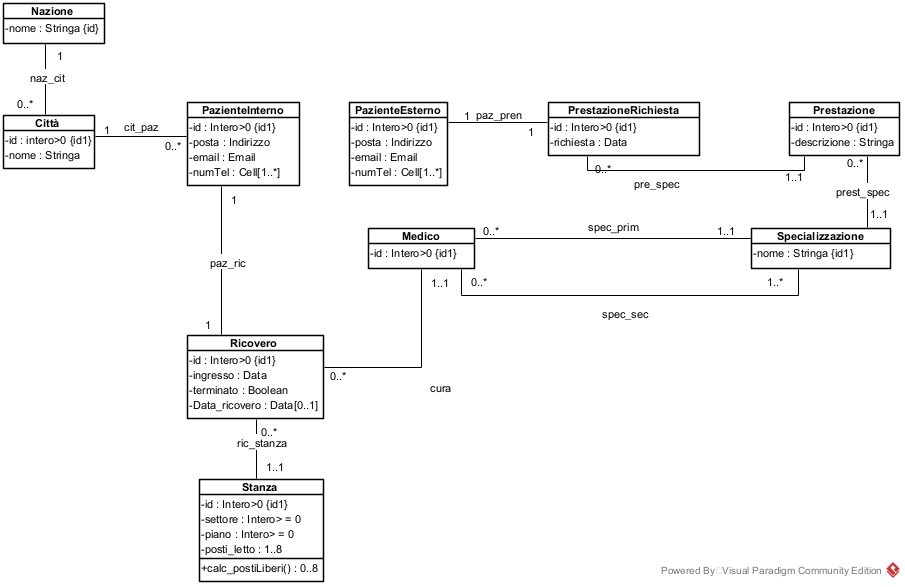
\includegraphics[width=1\textwidth ]{images/Ristrutturato.jpg}
\end{center}
\textbf{Modifiche sulle generalizzazioni effettuate:}
\begin{itemize}
    \item Generalizzazione PazienteEsterno$-$PazienteInterno: \\
    E' stata preferita la divisione tra pazienti interni ed esterni poichè è più facile e veloce nella ricerca avere due tabelle separate.\\
    Se un paziente è sia interno che esterno, avrò 2 tuple uguali sulle due tabelle.
    \item Generalizzazione Ricovero$-$RicoveroTerminato: \\
    La generalizzazione per RicoveroTerminao è stata eliminata.
    \item Generalizzazione SpecializzazionePrimaria$-$SpecializzazioneSecondaria: \\
    La generalizzazione tra SpecializzazionePrimaria e SpecializzazioneSecondaria è stata eliminata e aggiunto un vincolo esterno.\\

\end{itemize}

\newpage
\subsection{Tipi e Domini}
\subsubsection{Tipi}
\begin{itemize}
    
    \item create type Indirizzo as enum \{
        via: varchar(100),
        n$\_$civico: Intero$>$0,
    \}

\end{itemize}
\subsubsection{Domini}
\begin{itemize}
    \item create domain Intero$>$0 as integer check(value$>$0 not NULL)
    \item create domain Telefono as integer secondo regex ('$+[1..9]\{2\}$ $[0..9]\{10\}$')
    \item create domain Email as varchar secondo regex ('[a..zA..Z]@[a..z].[a..z]') 
\end{itemize}
\subsection{Vincoli Esterni}
I precedenti vincoli esterni non violano la nuova ristrutturazione.
Nuovi vincoli esterni:
\begin{itemize}
    \item Data Una SpecializzazionePrimaria essa non può essere SpecializzazioneSecondaria per lo stesso medico.\\
        $\forall m, s Medico(m) \land Specializzazione(s) \land SpecializzazionePrimaria(m,s)$\\ $\rightarrow \lnot SpecializzazioneSecondaria(m,s)$
\end{itemize}
\subsection{Use Case}
Gli use case non violano la nuova ristrutturazione.
\newpage
\subsection{Traduzione diretta del diagramma UML delle classi ristrutturato}
Saranno scritte tutte le tabelle da creare.
\begin{itemize}
    \item Nazione(\underline{\textbf{nome}}:varchar)
    \item Citta(\underline{\textbf{id}}:integer, nome:varchar)\\ v.inclusione: Città(Nome) occorre in $naz\_cit$(nazione)
    \item $naz\_cit$(\underline{\textbf{Nazione}}:varchar,\underline{\textbf{Citta}}:integer)\\
            foreign key: Nazione references Nazione(nome)\\
            foreign key: Citta references Citta(id)\\
    \item PazienteInterno(\underline{\textbf{id}}:integer, posta: Indirizzo, email: Email, numTel:Cell)\\
           v.inclusione PazienteInterno(id) occorre in $cit\_paz$(Paziente)
    \item $cit\_paz$(\underline{\textbf{Citta}}:varchar,\underline{\textbf{Paziente}}:integer)\\
            foreign key: Nazione references Paziente(id)\\
            foreign key: Citta references Citta(id)\\
    \item Ricovero(\underline{\textbf{id}}: integer, ingresso: Date, terminato: Boolean: $data\_ricovero$:Date*)\\
            v.inclusione Ricovero(id) occorre in $ric\_stanza$(Ricovero)
            v.inclusione Ricovero(id) occorre in $cura$(Ricovero)
    \item $paz\_ric$(\underline{\textbf{Paziente}}:integer,\underline{\textbf{Ricovero}}:integer)\\
    foreign key: Nazione references Paziente(id)\\
    foreign key: Citta references Ricovero(id)\\
    \item Stanza(\underline{\textbf{id}}: integer, settore: intero$>$0,piano: intero$>=$0 $posti\_letto: 1..8$)
    \item $ric\_stanza$(\underline{\textbf{Ricovero}}: intero,\underline{\textbf{Stanza}}:integer)\\
    foreign key: Ricovero references Ricovero(id)\\
    foreign key: Stanza references Stanza(id)\\
    \item PazienteEsterno(\underline{\textbf{id}}:integer, posta: Indirizzo, email: Email, numTel:Cell)
    \item PrenotazioneRichiesta(\underline{\textbf{id}}:integer, richiesta: Date)\\
            v.inclusione PrenotazioneRichiesta(id) occorre in $pre\_spec$(Prenotazione)
    \item $paz\_pren$(\underline{\textbf{Paziente}}:integer,\underline{\textbf{Prenotazione}}:integer)\\
            foreign key: Paziente references PazienteEsterno(id)\\
            foreign key: Prenotazione references PrenotazioneRichiesta(id)\\
\newpage
    \item Prenotazione(\underline{\textbf{id}}:integer, descrizione: varchar(100))\\
    v.inclusione Prenotazione(id) occorre in $prest\_spec$(Prenotazione)
    \item $pre\_spec$(\underline{\textbf{PrenotazioneRichiesta}}: integer,\underline{\textbf{Prenotazione}}: integer)\\
    foreign key: Prenotazione references Prenotazione(id)\\
    foreign key: PrenotazioneRichiesta references PrenotazioneRichiesta(id)\\
    \item Specializzazione(\underline{\textbf{nome}}: varchar(100))
    \item $prest_spec$(\underline{\textbf{Prenotazione}}: integer,\underline{\textbf{Specializzazione}}: varchar(100))\\
    foreign key: Prenotazione references Prenotazione(id)\\
    foreign key: Specializzazione references Specializzazione(varchar)\\
    
    \item Medico(\underline{\textbf{id}}: integer))\\
    v.inclusione Medico(id) occorre in $spec\_prim$(Medico)\\
    v.inclusione Medico(id) occorre in $spec\_sec$(Medico)
    \item $spec\_prim$(\underline{\textbf{Medico}}: intero,\underline{\textbf{Specializzazione}}: varchar(100))\\
    foreign key: Medico references Medico(id)\\
    foreign key: Specializzazione references Specializzazione(nome)\\
    \item $spec\_sec$(\underline{\textbf{Medico}}: intero,\underline{\textbf{Specializzazione}}: varchar(100))\\
    foreign key: Medico references Medico(id)\\
    foreign key: Specializzazione references Specializzazione(nome)\\
    \item cura(\underline{\textbf{Ricovero}}: intero,\underline{\textbf{Medico}}:integer)\\
    foreign key: Ricovero references Ricovero(id)\\
    foreign key: Medico references Medico(id)\\
    
\end{itemize}
\end{document}